\chapter{Power, Emergency Stop and Safety}
\label{ch:power}

The machine is switched on and off at the panel. LiNC follows: it shows the power and
emergency-stop state on every page, and it blocks machine-modifying actions while either
of them forbids motion.

\section{The power controls}

\begin{figure}[H]
  \centering
  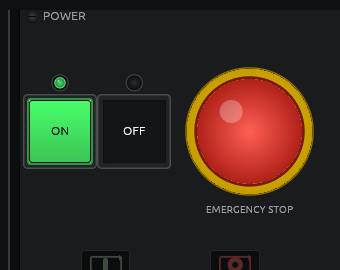
\includegraphics[width=0.42\textwidth]{img/crops/power.png}
  \caption{The power group: \textbf{ON} (lit green when machine power is on),
           \textbf{OFF}, and the emergency stop mushroom.}
  \label{fig:power}
\end{figure}

\begin{description}[font=\normalfont\sffamily\bfseries, leftmargin=3.4cm, style=nextline]
  \item[\pbtn{ON}] Switches machine power on and requests \emph{machine on} in the
        controller. Drives and outputs are enabled. The lamp in the key lights green.
  \item[\pbtn{OFF}] Switches machine power off. LiNC ends its session when the
        controller reports that machine power has dropped.
  \item[EMERGENCY STOP] The red mushroom. It latches when pressed and is released by
        turning it clockwise. See section~\ref{sec:estop}.
\end{description}

The simulator starts in the state a real cabinet is found in: emergency stop latched and
power off. Nothing moves until the mushroom is released and \pbtn{ON} is pressed. This is
deliberate: the power-up sequence is part of the training.

\section{Switching on}

\begin{enumerate}
  \item Check that the work area is clear, the guards are closed and no tool or clamp is
        left on the table.
  \item Release the emergency stop: turn the red mushroom clockwise until it pops out.
  \item Press \pbtn{ON}. The controller enables the drives.
  \item Wait for the panel's \ledlit{leddamber} \state{READY} lamp and for the interface
        to show \state{MACHINE ON} in the bottom bar.
  \item Home the axes (chapter~\ref{ch:modes}). \state{NOT HOMED} in the bottom bar means
        the controller has no valid reference, and no program will start.
  \item Load the program (chapter~\ref{ch:running}), check it, then run it from the panel.
\end{enumerate}

\begin{notebox}
  LiNC does not power the machine on and does not home it. Both are panel actions, wired
  to the controller through the machine's HAL. LiNC reports their state.
\end{notebox}

\section{Emergency stop}
\label{sec:estop}

\begin{safetybox}
  The emergency stop stops all axis motion, the spindle and the coolant immediately.
  Keep it reachable. Never bypass it, and never work around a machine that will not
  leave the emergency-stop state.
\end{safetybox}

Behaviour on this controller:

\begin{itemize}
  \item \textbf{Pressing} the mushroom latches the panel input. The controller enters
        emergency stop, drives are disabled and motion stops. LiNC shows the red banner
        \state{EMERGENCY STOP ACTIVE — MOTION AND MACHINE ACTIONS BLOCKED} on every page,
        and the bottom bar reads \state{E-STOP ACTIVE}.
  \item \textbf{Releasing} the mushroom clears the latch and asks the controller to leave
        emergency stop. It does \emph{not} switch machine power on: that is a separate
        \pbtn{ON} press. This separation is deliberate, so releasing the mushroom cannot
        start the machine.
  \item After a release, press \pbtn{ON} again if power dropped, check \state{READY}, and
        check the homing state before continuing.
\end{itemize}

\begin{cautionbox}
  An emergency stop interrupts the program mid-block. Before restarting, inspect the tool
  position and the remaining path. Use single block and a reduced feed override for the
  first blocks after recovery.
\end{cautionbox}

\section{Switching off}

\begin{enumerate}
  \item Finish or stop the running program (\pbtn{CYCLE STOP} on the panel).
  \item Unload the program with \chordtwo{Ctrl}{U} on the Program page if you are
        finished with it (section~\ref{sec:unload}).
  \item Press \pbtn{OFF}. The controller shuts down and LiNC ends its session.
\end{enumerate}

\begin{cautionbox}
  Do not cut the main disconnect while a program is running. Use \pbtn{OFF} first, so the
  controller can stop in a defined state.
\end{cautionbox}

LiNC refuses a normal quit (\chordtwo{Ctrl}{Q}) while a program is running or an
axis is moving. Losing machine power is the one case where the session ends regardless,
because the controller is going away anyway.

\section{Program protect}

\begin{figure}[H]
  \centering
  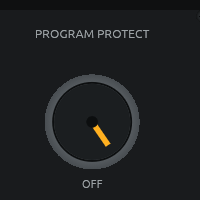
\includegraphics[width=0.24\textwidth]{img/crops/protect.png}
  \caption{The \textbf{PROGRAM PROTECT} key switch. \texttt{OFF} is the working position;
           \texttt{ON} locks every write.}
  \label{fig:protect}
\end{figure}

The panel's key switch is authoritative. While it is on, LiNC cannot:

\begin{itemize}
  \item edit the program buffer or save it,
  \item write an offset, a tool row or a tool length,
  \item copy or import a file into the program directory,
  \item apply a probe result to a work offset.
\end{itemize}

The screen shows the banner \state{PROTECT ON — EDITING LOCKED} on the pages that write,
and the field \state{PROTECT ON} in the bottom bar. Reading, loading and running a program
remain possible: protect blocks writing, not viewing.

\begin{notebox}
  Protect fails closed. If the switch state is unknown or the panel data is stale, LiNC
  treats protect as \emph{on}. Every write checks it again in the backend; a value the
  screen sampled earlier is not enough.
\end{notebox}

Unsaved edits are not thrown away when protect is switched on. The buffer stays, keeps
its dirty marker and becomes read-only until the switch returns to \texttt{OFF}.

\section{Limits override}

If an axis stands on a limit switch, the panel's jog keys are refused. The keyboard chord
\chordthree{Ctrl}{Shift}{O} toggles the controller's limit-switch override so
the axis can be jogged off the switch.

\begin{cautionbox}
  While the override is on, the limit switches are ignored and the machine can be driven
  past them. The screen shows a blinking \state{LIMITS OVERRIDE ON} in the bottom bar and
  the banner \state{LIMITS OVERRIDE ACTIVE — LIMIT SWITCHES ARE IGNORED}, but neither
  stops the machine. Jog off the switch, then switch the override off again.
\end{cautionbox}

\section{Panel offline and invalid mode}

LiNC reads the panel through the panel service. Two failures are shown as banners and
both fail closed:

\begin{description}[font=\normalfont\sffamily\bfseries, leftmargin=4.2cm, style=nextline]
  \item[\state{PANEL OFFLINE}] No current panel data. Machine-modifying actions are
        blocked, and the top bar's \state{PANEL} dot turns red.
  \item[\state{PANEL MODE INVALID}] The mode selector reports zero or more than one
        position. LiNC does not guess: the mode reads \state{UNKNOWN} and mode-dependent
        actions are refused until a valid position arrives.
\end{description}

The hardware emergency stop is independent of both. It works even when the panel service
is down, because it is wired in the machine's HAL.

\section{The external link interlock}
\label{sec:interlock}

On a machine whose only external network link is WiFi, LiNC can hold that link down while
the machine is able to move. WiFi association, driver interrupts and packet bursts all
cost realtime, and none of them are needed while a program runs.

\begin{notebox}
  The interlock only ever touches the external link named in the profile. The machine's
  internal fieldbus is never touched.
\end{notebox}

\textbf{When it is armed.} The link is held down while a program is loaded or the panel is
in \texttt{MDI}. It is released when nothing is loaded and no MDI block is being set up.
This is arm-on-intent, not arm-on-motion: a loaded program that is paused still holds the
link down, because it can be resumed.

\textbf{The \state{NET} field.} The top bar always shows the link state:

\begin{center}
\begin{tabular}{lll}
  \toprule
  \textbf{Value} & \textbf{Colour} & \textbf{Meaning} \\
  \midrule
  \state{DOWN} & green & Link down. This is the state the interlock wants while armed. \\
  \state{UP}   & muted & Link up, no program motion. Normal while setting up. \\
  \state{UP}   & amber & Link up \emph{and} program motion. The one state to look at. \\
  \state{MEAS} & accent & A link measurement is running. \\
  \state{?}    & amber & State unknown or stale. Fails closed. \\
  \state{OFF}  & muted & No interlock configured in this profile. \\
  \bottomrule
\end{tabular}
\end{center}

Amber is reserved for program motion on purpose. Jogging and homing keep the link up by
design, and colouring every setup jog amber would train the operator to ignore the one
colour that matters.

\textbf{Releasing the link.} Press \chordtwo{Ctrl}{U} on the Program page. LiNC
closes the program at the controller, resets the interpreter, re-reads the program name and
only then reports success. The \state{NET} field returns to \state{UP} within a few
seconds, after the radio has associated and a default route exists. A toast says
\state{UNLOAD REQUESTED — WATCH NET}.

\begin{cautionbox}
  Leaving a program loaded keeps the link down, and the link is the only remote way into
  the machine. If you need remote access while nothing is being cut, unload the program
  first. Profiles that must keep the link up can set \texttt{keep\_up = true} in
  \texttt{[network]}.
\end{cautionbox}

If the link is up while a program is loaded, commands that would run or change the program
are refused with \state{NETWORK BUSY} rather than being sent.

\section{Probe trip}

If the probe input rises during a move that is not a probe, the controller aborts the move
and reports an operator error. LiNC treats this as a latched fault, not a passing message:

\begin{itemize}
  \item A red banner carries the controller's own text on every page, for example
        \state{PROBE TRIPPED — … — MACHINE SWITCHED OFF. MOTION AND MDI BLOCKED. RESET
        (ESC) TO CLEAR.}
  \item The machine is switched off through \halpin{linc.machine-off}, so the panel cannot
        jog into the probe either. One exception exists: a trip raised with the program
        paused and nothing moving leaves the machine on, because nothing had to be stopped.
  \item MDI, probe, tool-change, jog-parameter and table writes fail closed until the trip
        is cleared.
  \item \keycap{Esc} (or the banner's \sbtn{RESET}) clears it, from any page. That sends the
        controller reset which clears the motion error. Re-powering afterwards needs a fresh
        \pbtn{ON}.
\end{itemize}

\section{Safety rules, in short}

The safety and liability disclaimer that applies to this software is printed at the front
of this manual, before the contents.

\begin{safetybox}
  \begin{itemize}
    \item The panel is the only place machine motion starts. Do not look for a jog or a
          cycle start on the screen.
    \item Release the emergency stop, then press \pbtn{ON}: two separate actions.
    \item Never leave the machine in limits override.
    \item Never run a program that shows red path outside the machine envelope without
          knowing why.
    \item Unload the program before relying on the network link.
  \end{itemize}
\end{safetybox}
